\documentclass[UTF8]{ctexart}
\usepackage{geometry}
\usepackage{anyfontsize}
%\usepackage[fontsize=10pt]{fontsize}
\usepackage{amsmath}
\usepackage{amssymb}
\usepackage{mathtools}
\usepackage{mathrsfs}
\usepackage{ntheorem}
\usepackage{xcolor}
\usepackage{bm}
\usepackage{listings}
\usepackage{graphicx}
\usepackage{booktabs}
\usepackage[ruled,linesnumbered]{algorithm2e}

\geometry{margin=1.2in}

\DeclareMathOperator*{\argmax}{\arg\!\max}
\DeclareMathOperator*{\argmin}{\arg\!\min}

\newtheorem{theorem}{定理}[section]
\newtheorem{corollary}[theorem]{推论}
\newtheorem{lemma}[theorem]{引理}
\newenvironment{proof}{{\textit{证明}:\quad }}{\hfill $\blacksquare$\par}

\lstset{
    basicstyle          =   \sffamily,          % 基本代码风格
    keywordstyle        =   \bfseries,          % 关键字风格
    commentstyle        =   \rmfamily\itshape,  % 注释的风格,斜体
    stringstyle         =   \ttfamily,  % 字符串风格
    flexiblecolumns,                % 别问为什么,加上这个
    numbers             =   left,   % 行号的位置在左边
    showspaces          =   false,  % 是否显示空格,显示了有点乱,所以不现实了
    numberstyle         =   \zihao{-5}\ttfamily,    % 行号的样式,小五号,tt等宽字体
    showstringspaces    =   false,
    captionpos          =   t,      % 这段代码的名字所呈现的位置,t指的是top上面
    frame               =   lrtb,   % 显示边框
}

\lstdefinestyle{Python}{
    language        =   Python % 语言选Python
    basicstyle      =   \zihao{-5}\ttfamily,
    numberstyle     =   \zihao{-5}\ttfamily,
    keywordstyle    =   \color{blue},
    keywordstyle    =   [2] \color{teal},
    stringstyle     =   \color{magenta},
    commentstyle    =   \color{red}\ttfamily,
    breaklines      =   true,   % 自动换行,建议不要写太长的行
    columns         =   fixed,  % 如果不加这一句,字间距就不固定,很丑,必须加
    basewidth       =   0.5em,
}

\begin{document}

\title{流形优化期末报告}
\author{张晨}
\date{2024年9月23日}
\maketitle

\section{Question 1}

\section{Question 2}

编程实现教材上的Algorithm 3和Algorithm 4, 随机生成Stiefel流形的一个二次函数, 用Algorithm 4极小化这个二次函数, 比较两个算法的计算效果, 探索非单调的作用, 或者交替使用BB步长两个公式的作用. \par

\subsection{随机二次函数的生成}

首先考虑实现二次函数的随机生成问题. 对于整数$n\geq p>0$, 欧氏空间$\mathbb{R}^{n\times p}$上的$Stiefel$流形为
\[\textup{St}(n,p)=\{X\in\mathbb{R}^{n\times p}|X^T X=I_p\}.\]
对于矩阵$B\in \mathbb{R}^{n\times p}$和对称正定矩阵$A\in\mathbb{R}^{n\times n}$, $St(n,p)$上的二次函数定义为
\[f(X;A,B)=\textup{tr}(X^T AX+2X^T B).\]
故二次函数$f$的生成问题等价于矩阵$A,B$的生成问题. 在MATLAB中, 可以使用\textbf{randn}函数随机生成矩阵, 因此, 可以取
\[B\leftarrow \textup{randn}(n,p).\]
但MATLAB中并没有直接生成对称正定矩阵的函数. 为了随机生成$A$, 先考虑一个简单的引理: 
\begin{lemma}
    记集合$\mathcal{A}$为对称正定矩阵全体, 定义集合
    \[\mathcal{B}=\{R^T R+D|R\in\mathbb{R}^{n\times n}, D=\textup{diag}(d_1,\cdots,d_n), 0<d_1,\cdots,d_n<1\},\]
    则$\mathcal{A}=\mathcal{B}$. 
\end{lemma}
\begin{proof}
    首先证明$\mathcal{B}\subseteq\mathcal{A}$. 对于任意的$B=R^T R+D\in\mathcal{B}$, 有
    \[B^T=(R^T R+D)^T=R^T R+D^T=R^T R+D=B,\]
    故$B$是对称的. 对于任意的$x\in\mathbb{R}^n_*$, 有
    \[x^T Bx=(Rx)^T(Rx)+x^T Dx\geq x^T Dx\geq d_1 \lVert x\rVert_2^2>0.\]
    因此, $B\in\mathcal{A}$.\par
    再证明$\mathcal{A}\subseteq\mathcal{B}$. 对于任意的$A\in\mathcal{A}$, 记$\lambda>0$为$A$的最小特征值, 取$d=\min(\lambda/2,1/2)$, 则矩阵$A-dI_n$仍为对称正定矩阵. 注意到, 根据对称正定矩阵的Cholesky分解, 存在矩阵$R\in\mathbb{R}^{n\times n}$, 使得
    \[A=(A-dI_n)+dI_n=R^T R+dI_n\in\mathcal{B}.\]
    综上, $\mathcal{A}=\mathcal{B}$. 
\end{proof}\par
根据这个引理, 结合MATLAB中取值在$(0,1)$上的随机函数\textbf{rand}, 可以得到对称正定矩阵的随机生成方法:
\begin{align*}
    R&\leftarrow \textup{randn}(n,n),\\
    A&\leftarrow R^T R+\textup{diag}(\textup{rand}(n)). 
\end{align*}\par
详细的代码实现可以参考附录. 在下文中, 我们考虑$n=500$, $p=50$时各算法的表现, 取MATLAB中随机函数的种子为$99$, 生成的矩阵对$(A,B)$同样可见附录.

\subsection{梯度下降算法与BB算法的比较}

本小节中, 我们使用基于单调线搜索的梯度下降算法与基于非单调线搜索的BB算法对二次函数$f(X)=\textup{tr}(X^T AX+2X^T B)$进行优化. 在参数选择上, 我们使用表\ref{tab1}中的参数值. \par
\begin{table}[htbp]
    \centering
    \begin{tabular}{c|cc}
        \hline
        \hline
        参数 & 具体数值 & 参数描述\\
        \hline
        $t_0$ & $0.02$ & 回退法的初始步长\\
        $\rho$ & $0.5$ & 回退幅度\\
        $c$ & $0.001$ & Armijo条件的系数\\
        $M$ & $5$ & 非单调线搜索的前项个数\\
        $\alpha_{\max}$ & $100$ & BB步长的上界\\
        $\alpha_{\min}$ & $0.01$ & BB步长的上界\\
        \hline
        \hline
    \end{tabular}
    \caption{算法参数}\label{tab1}
\end{table}
我们先分析一下两个算法的收敛速度, 随机选取初始点$X_0$, 在算法中使用基于QR分解的收缩映射, 观察函数值$f(X_k)$与点列$X_k$的误差变化情况, 结果见图\ref{fig1}, 其中左图为函数值$f(X_k)$的相对误差随迭代次数的变化情况, 右图为点列$X_k$关于极小值点$X^*$的相对误差, 其度量为两点作为$\mathbb{R}^{n\times p}$矩阵时, 差值$X_k-X^*$的Frobenius范数. \par
\begin{figure}[htbp]
    \centering
    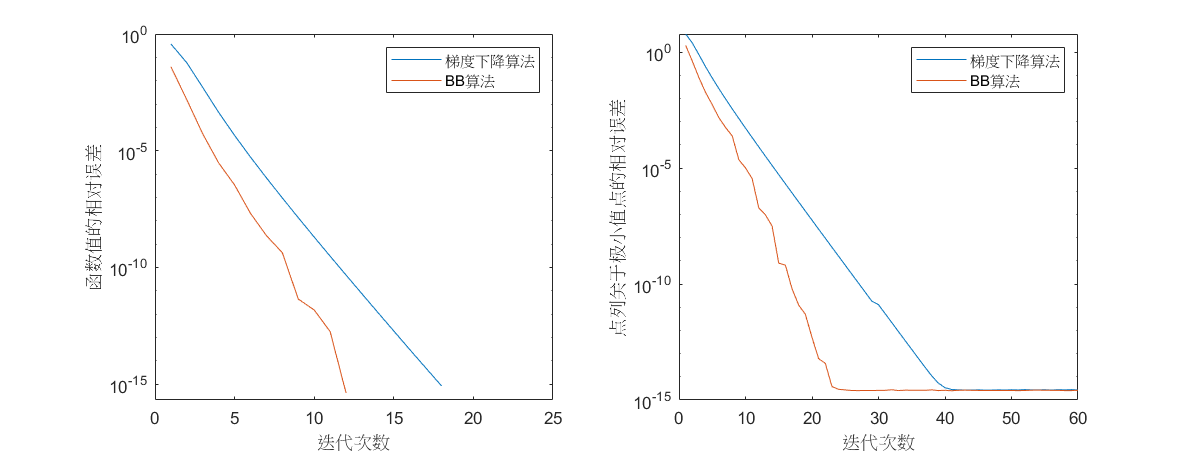
\includegraphics[width=0.7\textwidth]{Q2-figure/1.png}
    \caption{相对误差的变化情况}\label{fig1}
\end{figure}
从图\ref{fig1}中可以看出: 首先, 两个算法都在$50$步内迭代到了最小值点, 误差达到了机器精度; 其次, 这两个算法的收敛速度都是线性收敛, 且BB算法的速度要显著快于梯度下降算法; 最后, 函数值的收敛速度比点列的收敛速度更快, 这一点是由二次函数的性质产生的. \par
接下来, 对于不同的收缩映射算法, 我们对比一下算法的收敛速度, 结果见图\ref{fig2}, 其中左图均为函数值的相对误差变化情况, 右图均为点列的相对误差变化情况, 第一行为使用梯度下降算法得到的误差变化图, 第二行为使用BB算法得到的误差变化图. \par
\begin{figure}[htbp]
    \centering
    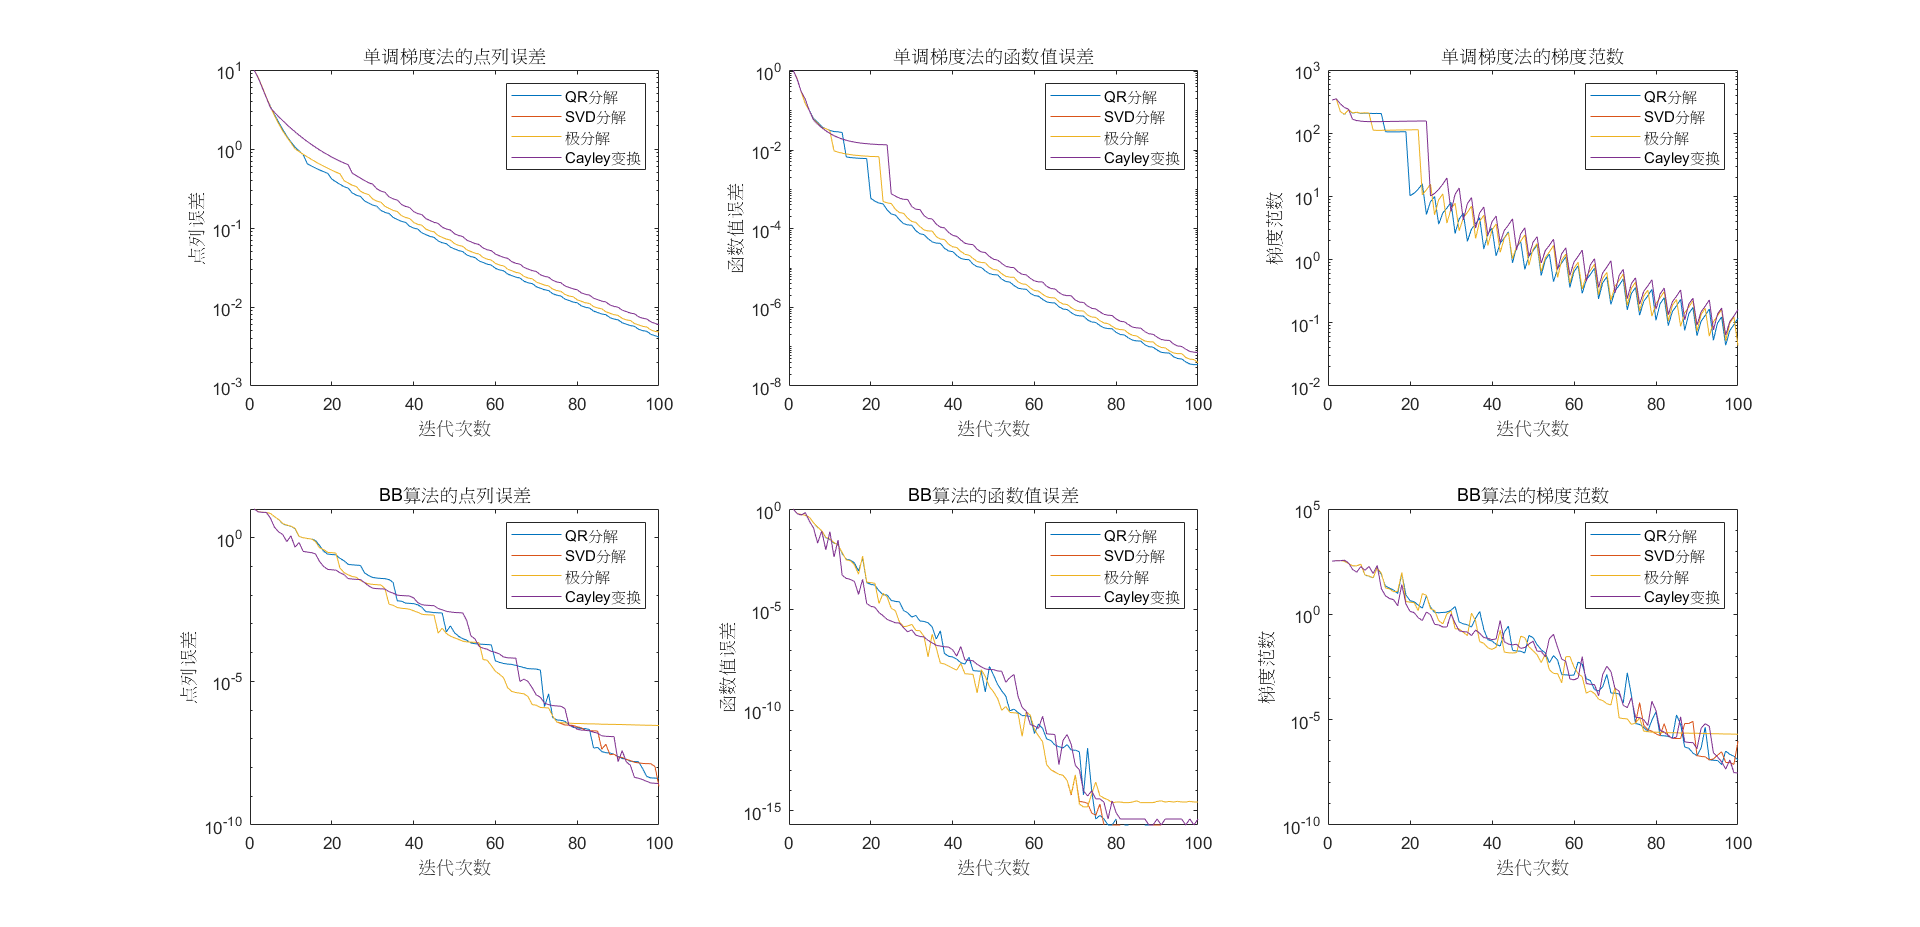
\includegraphics[width=0.7\textwidth]{Q2-figure/2.png}
    \caption{不同收缩映射算法的表现}\label{fig2}
\end{figure}
从图\ref{fig2}中可以看到, 不同收缩映射算法在函数值上的表现是相同的, 以同样的速度线性收敛. 值得一提的是, 基于Cayley变换的收缩映射算法会导致BB算法在前几次迭代的效果略差, 但在之后的迭代中仍然获得了和其他收缩映射算法相同的收敛速度. 当考察自变量$X$的收敛情况时, 不同的收缩映射算法产生了不同的表现. 在BB算法中, 基于Cayley变换的收缩映射算法仍然在前几次迭代中表现略差, 不过在长期迭代中, 这些收缩映射的表现是类似的; 但在梯度下降算法中, 基于QR分解和Cayley变换的收缩映射算法很快到达了机器精度, 基于SVD分解的收缩映射算法在20次迭代后放缓了收敛速度, 基于极分解的收缩映射算法只能达到$10^{-6}$精度, 无法达到机器精度. \par
值得特别一提的是, 在理论上, 基于SVD分解的收缩映射和基于极分解的收缩映射应当是同一个, 但这两种不同的收缩映射在梯度下降算法下的表现是不同的, 这可能是计算误差导致的: 在实现基于SVD分解的收缩映射时, 我们直接使用了MATLAB内置的\textbf{svd}函数, 这一函数是使用商业库MKL构建的, 因此会进行专业的优化, 达到比极分解更好的表现. \par
在下一节中, 我们将进一步讨论不同收缩映射的不同表现. 

\subsection{梯度下降算法中非单调线搜索的作用}


\end{document}